\documentclass[11pt,a4paper]{article}
\usepackage{iftex}
\ifXeTeX
  \usepackage{fontspec}
\else
  \usepackage[utf8]{inputenc}
  \usepackage[T1]{fontenc}
  \usepackage{lmodern}
\fi
\usepackage[french]{babel}
\usepackage[margin=2.3cm]{geometry}
\usepackage{amsmath,amssymb}
\usepackage{graphicx}
\usepackage{booktabs,tabularx}
\usepackage{xcolor}
\usepackage{enumitem}
\usepackage{listings}
\usepackage{fancyhdr}
\usepackage{microtype}
\usepackage{hyperref}
\hypersetup{colorlinks=true,linkcolor=teal!60!black,urlcolor=teal!60!black,
 pdftitle={TP n° 3 — Intégration SLAM},
 pdfauthor={Adib OUAMOU}}
\graphicspath{{figures/}}
\setlength{\parskip}{5pt}
\setlength{\parindent}{0pt}
\setlength{\emergencystretch}{2em}
\setlist[itemize]{nosep,leftmargin=*}
\pagestyle{fancy}
\fancyhf{}
\fancyhead[L]{TP n° 3 — Intégration SLAM}
\fancyhead[R]{Adib OUAMOU}
\fancyfoot[C]{\thepage}
\setlength{\headheight}{14pt}
\lstset{basicstyle=\ttfamily\footnotesize,breaklines=true,
 frame=single,backgroundcolor=\color{gray!5},columns=fullflexible,
 keepspaces=true,showstringspaces=false}
\newcommand{\code}[1]{\texttt{\detokenize{#1}}}

\begin{document}
\pagenumbering{Alph}
\begin{titlepage}
\centering
\vspace*{1.8cm}
{\Large EIGSI\par}
\vspace{0.5cm}
{\large Cartographie et localisation appliquées à la robotique mobile\par}
\vspace{2cm}
{\Huge\bfseries Rapport de TP n° 3\par}
\vspace{0.7cm}
{\LARGE Intégration SLAM\\à partir de mesures LiDAR\par}
\vspace{0.9cm}
{\large Localisation et cartographie simultanées,\\carte complète de la salle\par}
\vfill
{\large Auteur\par}
\vspace{0.2cm}
{\LARGE\bfseries Adib OUAMOU\par}
\vspace{1cm}
{\large 4 novembre 2026\par}
\vspace{1cm}
\end{titlepage}

\pagenumbering{roman}
\begingroup
\setlength{\parskip}{0pt}
\tableofcontents
\endgroup
\newpage
\pagenumbering{arabic}

\section*{Introduction}
\addcontentsline{toc}{section}{Introduction}
Les consignes du TP n° 3 demandent de combiner les outils des TP précédents
pour obtenir un système capable de localisation, puis de produire une carte
complète de la salle de classe. Elles invitent aussi à essayer de déplacer
le robot automatiquement pour construire la carte en temps réel ; cette
dernière partie est traitée comme un bonus (section~\ref{sec:bonus}).

Le système réalisé est un SLAM 2D incrémental (\emph{Simultaneous
Localization And Mapping}) : chaque scan est d'abord localisé par rapport à
ce qui a déjà été cartographié, puis intégré à la carte avec la pose obtenue.
Il réutilise directement :
\begin{itemize}
\item du TP n° 1 : la grille d'occupation (\code{gridmap.py}), l'extraction
de segments et la carte vectorielle (\code{segments.py}, \code{vectormap.py}) ;
\item du TP n° 2 : l'ICP en deux phases (\code{localisation_scans.py}) et le
recalage sur champ de distance de la grille (\code{localisation_grid.py}).
\end{itemize}

Deux SLAM sont comparés sur les mêmes données : le SLAM \emph{principal}
(\code{slam.py}), à graphe de poses, et une \emph{variante} plus simple
(\code{slam_carte.py}), à recalage direct sur la carte.

\section{Données et conventions}
Les douze scans réels du TP n° 1 ont été acquis dans la salle de classe
(fichiers \code{scan_*.csv}, 453 à 455 points chacun ; la fusion du TP n° 1
porte le nom \code{chambre_fusionnee}). Les poses utilisent le repère du
projet : $x$ et $y$ en mètres, $\theta$ en degrés dans le sens antihoraire.

Aucune pose physique n'a été mesurée. Les poses estimées hors ligne au
TP n° 1 par ICP multidépart (\code{alignements.json}) servent de
\emph{référence estimée} pour le rejeu réel : un écart à cette référence
mesure la cohérence entre deux méthodes, pas une erreur physique.
La précision est donc évaluée en simulation, où les poses vraies sont connues.

\section{SLAM principal : graphe de poses}
\subsection{Traitement d'un scan}
\begin{enumerate}[nosep]
\item \textbf{Filtrage} : distances entre 0,12 m et 20 m, sous-échantillonnage
par voxels de 5 cm, rejet des scans dégénérés (points alignés) ; les impacts
à moins de 0,60 m (châssis, objets très proches) restent dans la carte mais
ne servent pas au recalage.
\item \textbf{Prédiction} : la pose précédente, composée avec le déplacement
commandé quand il est connu (odométrie).
\item \textbf{Recalage ICP} sur une sous-carte : les points des huit images
clés les plus proches, dans le repère monde. En rejeu discontinu, l'ICP est
lancé depuis douze orientations ; un résultat est refusé s'il est ambigu
(deux solutions de qualité voisine et éloignées).
\item \textbf{Contrôle de qualité} : au moins 65\,\% des points à moins de
20 cm de la sous-carte, et résidu RMS des inliers $\le 0{,}10$ m.
\item \textbf{Affinage sur la grille} (recherche du TP n° 2 dans une fenêtre
de $\pm6$ cm et $\pm1{,}5^\circ$), conservé seulement s'il reste cohérent
avec la sous-carte ICP.
\item \textbf{Intégration} : mise à jour de la grille d'occupation (TP n° 1)
avec la pose retenue. Un scan refusé ne modifie pas la carte.
\end{enumerate}

\subsection{Images clés et fermeture de boucle}
Une image clé est créée après 25 cm ou $12^\circ$ de déplacement. Chaque
nouvelle image clé est comparée aux images clés anciennes et proches
(à moins de 0,9 m, après au moins 1,5 m de trajet) : un ICP direct puis
inverse doit donner deux transformations cohérentes (écart $\le 8$ cm et
$3^\circ$). La contrainte de boucle est alors ajoutée au graphe.

\subsection{Optimisation du graphe}
Les poses des images clés $\mathbf x_i=(x_i,y_i,\theta_i)$ minimisent la
somme des écarts entre les déplacements relatifs prédits et mesurés, pour
chaque contrainte $(a,b)$ séquentielle ou de boucle :
\[
 \min_{\mathbf x_1,\dots,\mathbf x_n}\sum_{(a,b)}
 \rho\Bigl(\bigl\|\Sigma^{-1/2}\bigl(R_{\theta_a}^{\top}(\mathbf t_b-\mathbf t_a)
 \ominus\mathbf z_{ab}\bigr)\bigr\|^2\Bigr),
\]
avec $\Sigma^{1/2}=\mathrm{diag}(6\text{ cm},6\text{ cm},2^\circ)$, une perte robuste
$\rho$ (\emph{soft L1}) et la première pose fixée. Les pondérations sont
heuristiques : elles ne proviennent pas d'une covariance mesurée.

\section{Améliorations apportées au SLAM}
La première version du SLAM a été profilée et évaluée, puis corrigée.
Chaque modification répond à un défaut mesuré.

\begin{table}[htbp]
\centering
\caption{Défauts mesurés et corrections.}
\begin{tabularx}{\linewidth}{>{\raggedright\arraybackslash}X>{\raggedright\arraybackslash}X}
\toprule
Défaut mesuré & Correction \\
\midrule
78\,\% du temps dans l'optimisation : la carte était reconstruite depuis
tous les scans après chaque boucle (38 millions d'appels Bresenham sur
150 pas) ; jacobienne dense (8 s). &
Résidus vectorisés et jacobienne creuse ; carte reconstruite depuis les
images clés, et seulement si la correction dépasse une demi-cellule ou
$0{,}5^\circ$ ; tracé de rayons vectorisé (TP n° 1). \\
Un scan refusé faisait perdre le déplacement déjà effectué. &
La pose suit la prédiction d'odométrie (navigation à l'estime). \\
Dérive : 75\,\% seulement des cellules occupées sur un vrai mur, et
jusqu'à 45 cm d'erreur en exploration. &
Affinage de chaque pose sur la grille, validé contre la sous-carte ICP. \\
Affinage piégé par un faux minimum (mobilier répétitif). &
Affinage refusé s'il dégrade le recouvrement ou le résidu ICP. \\
ICP point-à-point sensible à l'échantillonnage. &
ICP en deux phases du TP n° 2 (point-à-ligne en fin de convergence). \\
\bottomrule
\end{tabularx}
\end{table}

\section{Variante : recalage scan-sur-carte}
La variante \code{slam_carte.py} sert de point de comparaison. Elle n'a ni
images clés ni graphe : chaque scan est recalé directement sur la grille
construite avec tous les scans précédents, par la recherche hiérarchique du
TP n° 2 ($\pm30$ cm, $\pm10^\circ$ autour de la prédiction ; $\pm3$ m,
$\pm180^\circ$ en rejeu). Le scan est accepté si 60\,\% de ses points sont
à moins de 20 cm d'un obstacle de la carte. Elle est plus simple, mais ne
peut pas corriger une erreur ancienne : une dérive reste figée dans la carte.

\section{Protocole d'évaluation}
Les deux SLAM reçoivent exactement les mêmes données :
\begin{itemize}
\item \textbf{A. Trajet imposé en simulation} : deux salles simulées (une
salle simple de $10\times8$ m et une salle de classe de $9\times7$ m avec
sept tables), un trajet en boucle de 199 et 233 scans, scans de 450 rayons
(bruit radial de 1 cm, portée 12 m), odométrie bruitée (5\,\% sur les
distances et les angles, dérive latérale et angulaire). Trois graines.
\item \textbf{B. Exploration autonome simulée} (bonus) : chaque SLAM avec son
explorateur, au plus 250 pas, deux graines.
\item \textbf{C. Rejeu des douze scans réels} de la salle, dans le même ordre,
en partant du scan de référence de la fusion du TP n° 1.
\end{itemize}
Indicateurs : erreur de position et d'angle par rapport à la pose vraie
(A, B), part des murs vrais retrouvés et part des cellules occupées situées
à moins de 10 cm d'un vrai mur (A, B), surface couverte (B), scans acceptés
et écart à la référence estimée (C).

\section{Résultats}
\subsection{Simulation à poses connues}
\begin{table}[htbp]
\centering
\caption{Trajet imposé, moyennes sur trois graines. Pour référence,
l'odométrie seule dérive de 43 à 44 cm en moyenne (jusqu'à 1,17 m).}
\begin{tabular}{llrrrrr}
\toprule
Salle & SLAM & $e_t$ moy. & $e_t$ max & $e_\theta$ moy. & Cellules justes & Temps/scan \\
\midrule
Simple & Principal (avant) & 6,3 cm & 14,3 cm & $0,79^\circ$ & 93\,\% & 161 ms \\
Simple & \textbf{Principal} & \textbf{2,8 cm} & 4,5 cm & $\mathbf{0,11^\circ}$ & 100\,\% & 243 ms \\
Simple & Variante & 3,4 cm & 4,3 cm & $0,06^\circ$ & 100\,\% & 204 ms \\
\midrule
Classe & Principal (avant) & 15,3 cm & 37,3 cm & $2,22^\circ$ & 75\,\% & 86 ms \\
Classe & \textbf{Principal} & \textbf{5,3 cm} & 8,7 cm & $\mathbf{0,47^\circ}$ & 96\,\% & 197 ms \\
Classe & Variante & 5,9 cm & 9,7 cm & $0,52^\circ$ & 97\,\% & 174 ms \\
\bottomrule
\end{tabular}
\end{table}

Après correction, le SLAM principal divise l'erreur de position par 2 à 3
et l'erreur angulaire par 5 à 7 ; 96 à 100\,\% des cellules occupées sont
sur un vrai mur. Il est au niveau de la variante, et la dépasse en fin de
trajet grâce aux fermetures de boucle : erreur finale de 0,3 à 0,9 cm dans
la salle simple, contre environ 3,5 cm pour la variante. Le surcoût de
temps vient de l'affinage sur la grille et de la phase point-à-ligne ; il
reste compatible avec un scan par arrêt du robot.

\begin{figure}[htbp]
\centering
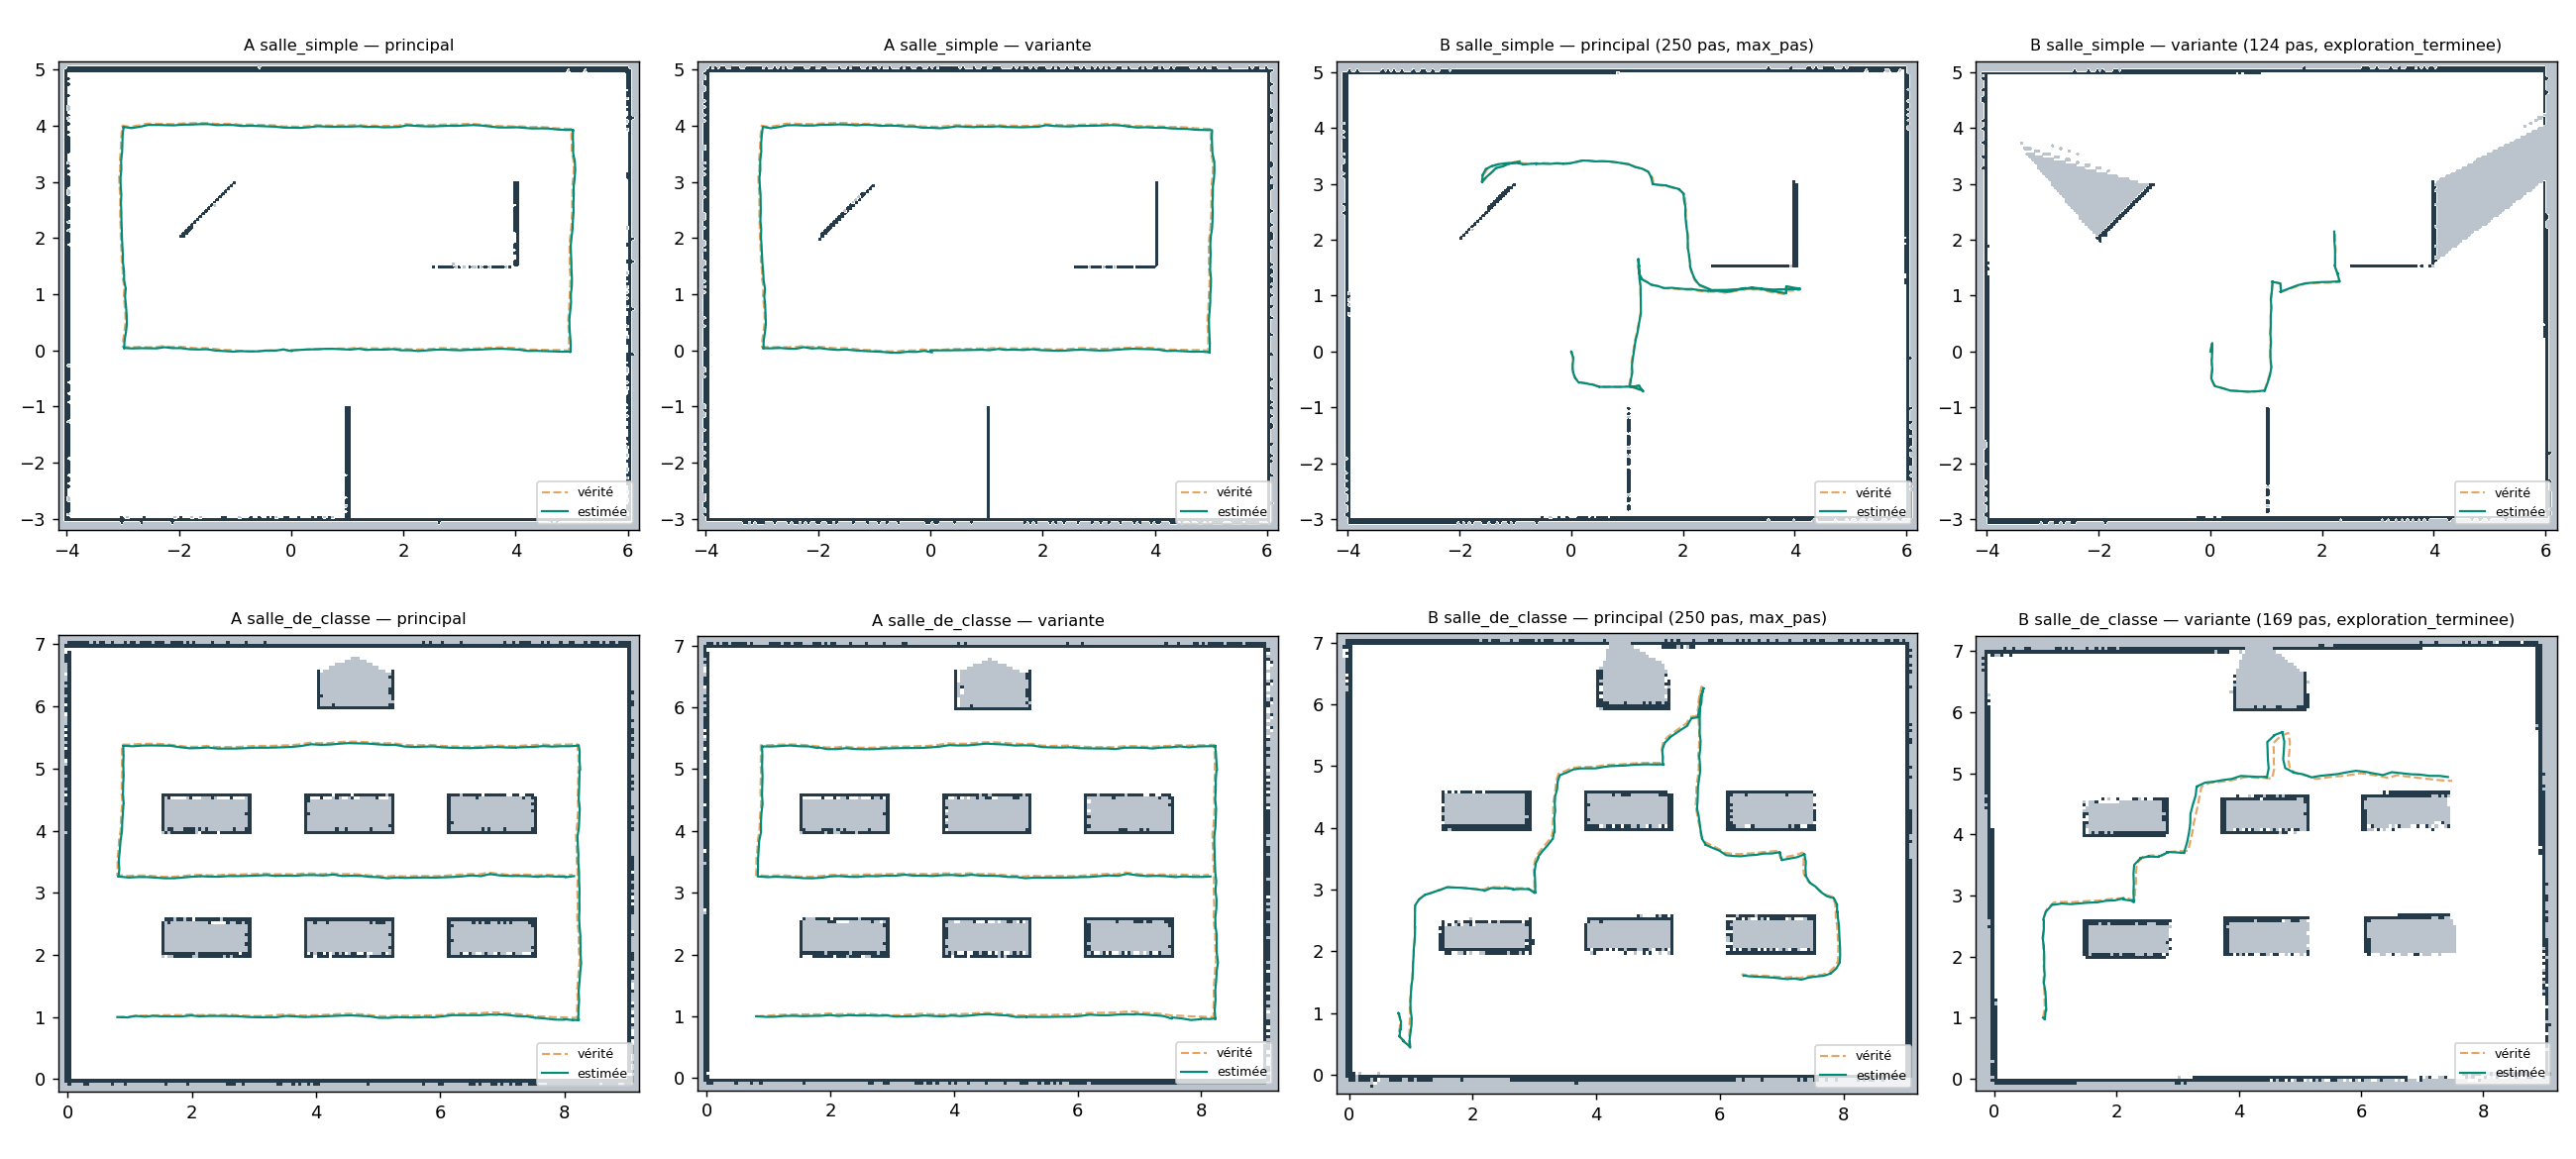
\includegraphics[width=\linewidth]{comparaison_simulation.png}
\caption{Simulation. Colonnes 1--2 : trajet imposé (pointillés orange :
trajectoire vraie ; vert : trajectoire estimée). Colonnes 3--4 : exploration
autonome. Gris : inconnu ; blanc : libre ; bleu foncé : occupé.}
\end{figure}

\subsection{Carte complète de la salle de classe}
Le rejeu des douze scans réels par le SLAM principal intègre huit scans ;
la carte obtenue (figure~\ref{fig:salle}) couvre la salle entière,
d'environ $8\times13$ m, avec 1\,053 cellules occupées, 45\,107 cellules
libres et 31 segments dans la carte vectorielle. Les murs sont rectilignes
et continus ; l'ouverture de la porte apparaît à droite, où les rayons
sortent de la salle.

\begin{figure}[htbp]
\centering
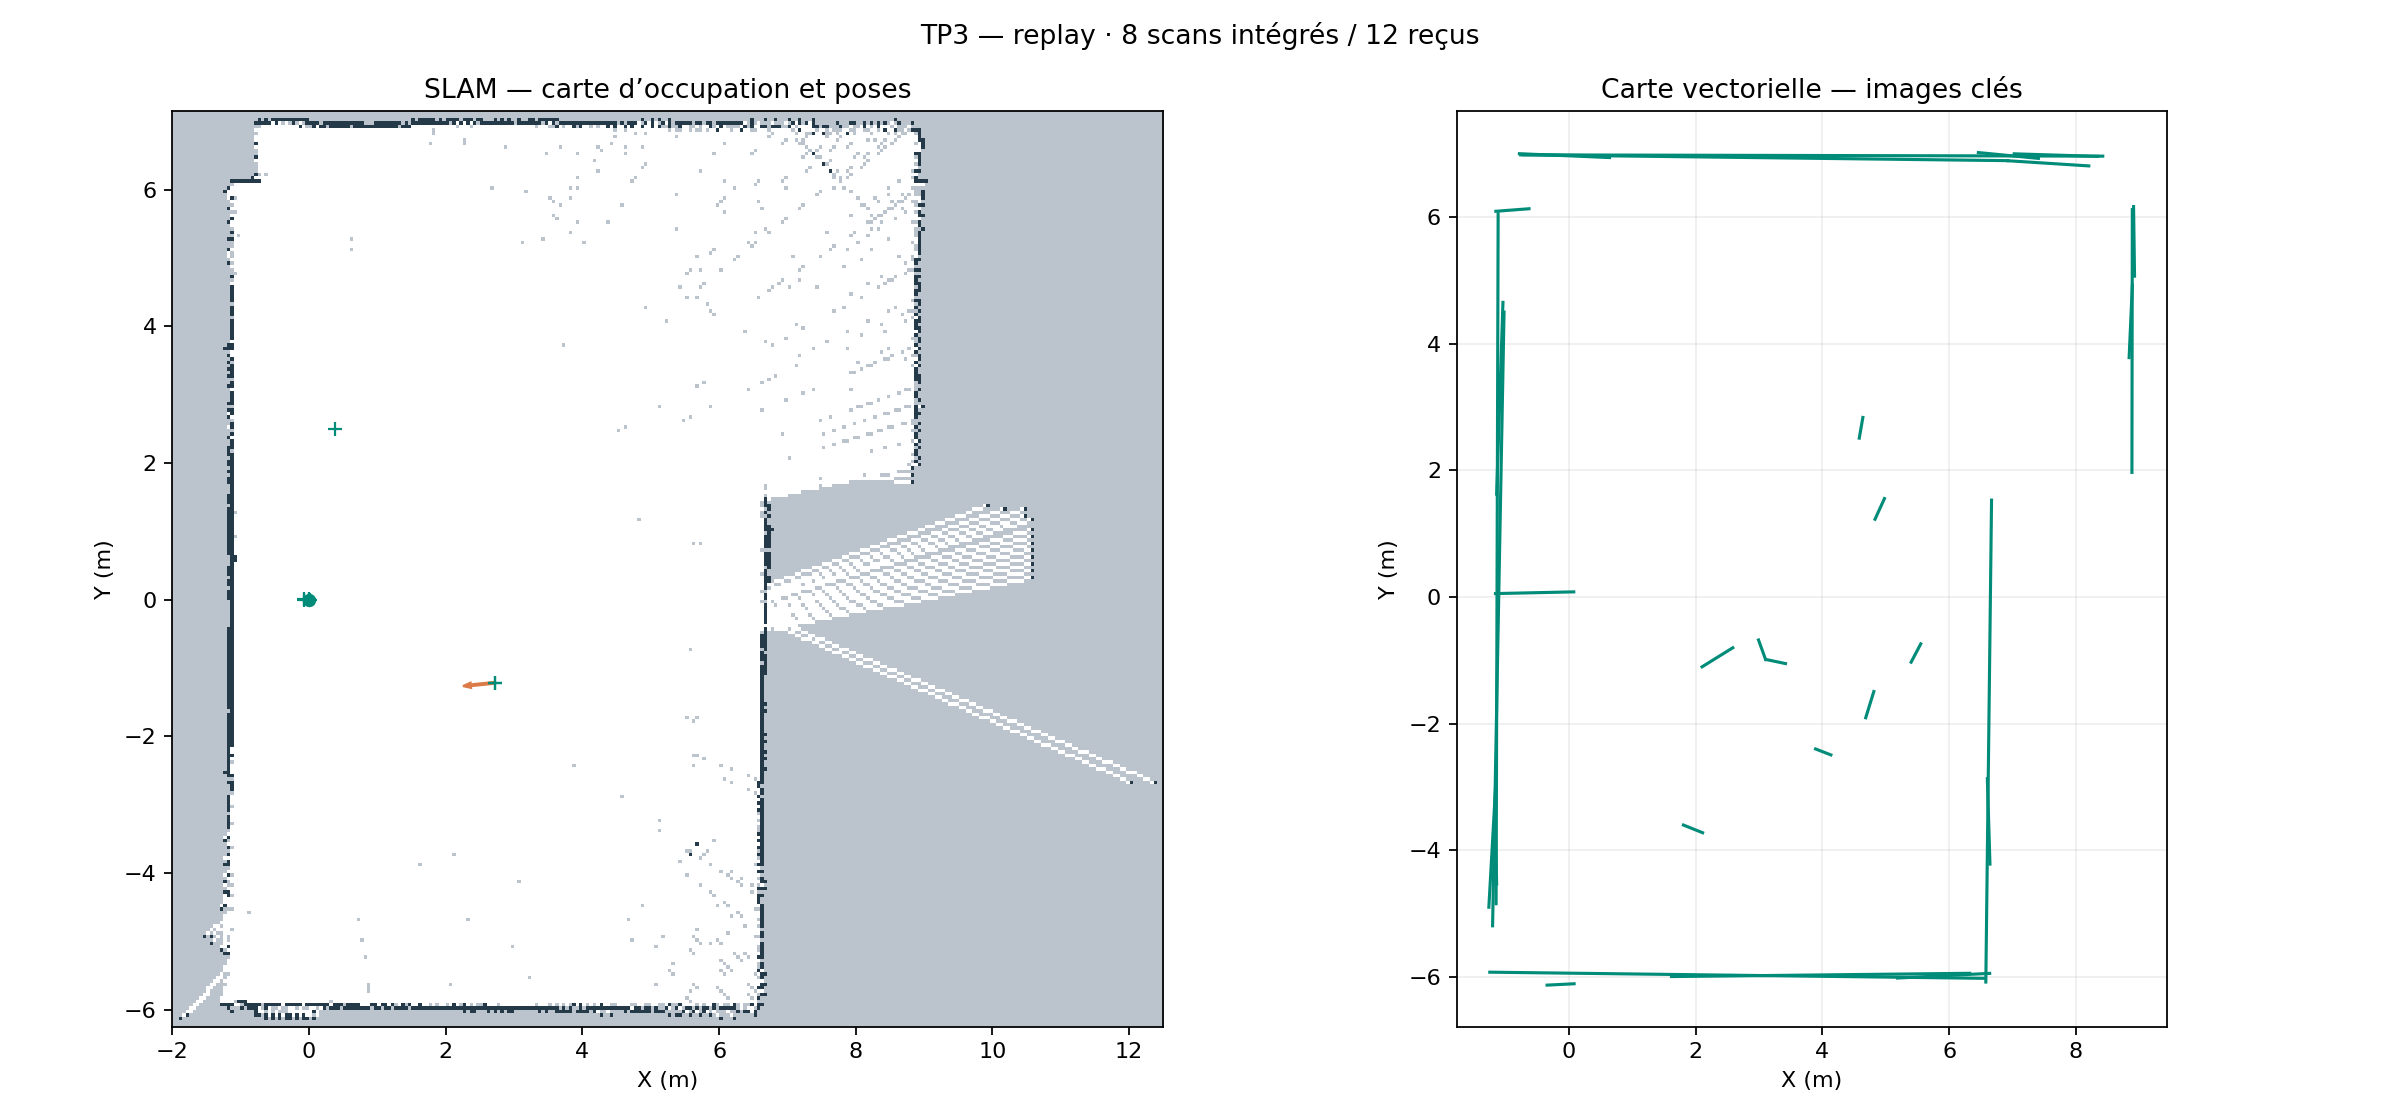
\includegraphics[width=\linewidth]{carte_salle_slam.png}
\caption{Salle de classe : carte d'occupation construite par le SLAM
principal à partir des scans réels (gauche ; croix : poses des scans
intégrés) et carte vectorielle extraite des images clés (droite).}
\label{fig:salle}
\end{figure}

\begin{table}[htbp]
\centering
\caption{Rejeu des douze scans réels. Écart = distance à la pose estimée
hors ligne au TP n° 1, qui n'est pas une vérité terrain.}
\begin{tabular}{lrrr}
\toprule
SLAM & Scans acceptés & Écart de position & Écart angulaire \\
\midrule
Principal & 8/12 & 0,7 à 2,5 cm & $0,13$ à $0,70^\circ$ \\
Variante & 9/12 & 2,2 à 6,9 cm & $0,10$ à $1,02^\circ$ \\
\bottomrule
\end{tabular}
\end{table}

Les quatre scans refusés sont les deux essais de 12~h~44 et 12~h~52
(acquis avant la série principale ; le premier a une distance médiane de
0,41 m seulement, le robot étant très près d'un obstacle), puis les scans de
17~h~00 et 17~h~09 ; ni l'ICP multidépart ni la recherche large sur la grille
n'y trouvent un recalage assez sûr. Le SLAM principal préfère refuser un scan
plutôt que de l'intégrer avec une pose douteuse : la carte reste propre,
au prix de zones vues par ces seuls scans. La variante accepte un scan de
plus mais s'écarte davantage de la référence.

\begin{figure}[htbp]
\centering
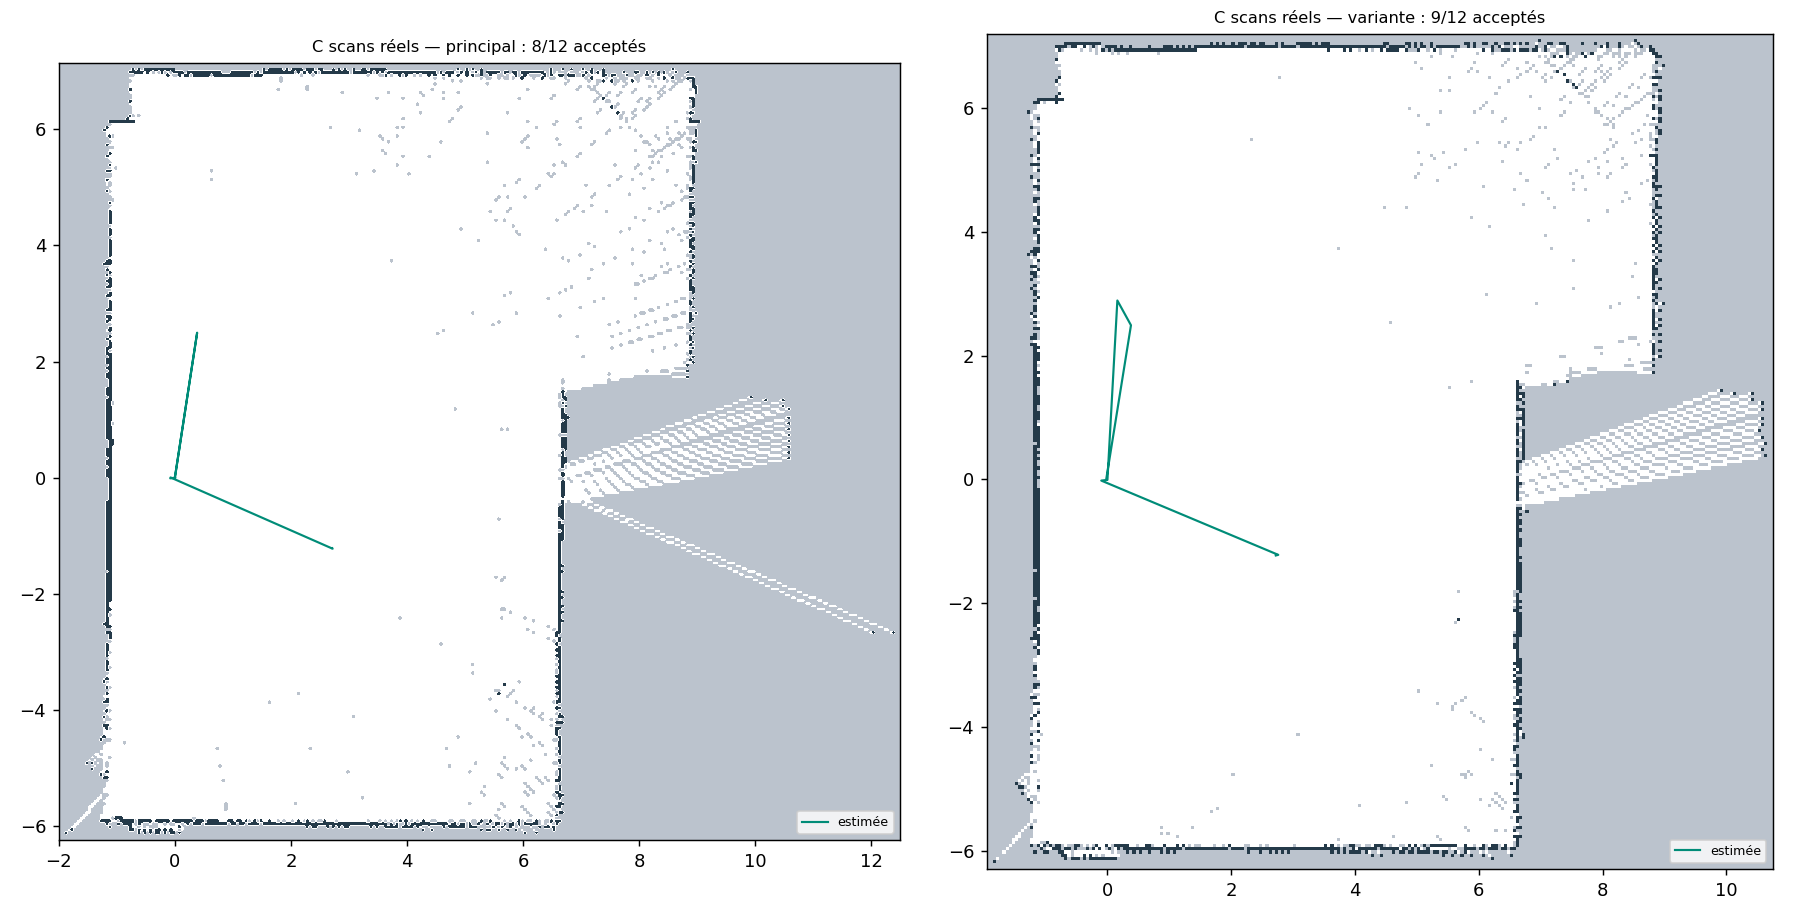
\includegraphics[width=\linewidth]{comparaison_scans_reels.png}
\caption{Rejeu des scans réels par les deux SLAM, dans les mêmes conditions.}
\end{figure}

\section{Bonus : exploration automatique}\label{sec:bonus}
\subsection{Explorateur par frontières}
Les frontières sont les cellules libres voisines de cellules inconnues,
regroupées en amas d'au moins trois cellules. L'explorateur :
\begin{itemize}
\item calcule la zone praticable : cellules libres à au moins 28 cm d'un
obstacle (rayon du robot 18 cm et marge 10 cm) ;
\item cherche par parcours en largeur la frontière accessible la plus proche ;
\item vise le point le plus lointain du chemin (40 cm au plus) visible en
ligne droite dans la zone praticable ;
\item tourne par pas de $25^\circ$ au plus, avance par pas de 12 cm ;
\item abandonne une frontière non atteinte après 40 actions, ou atteinte
sans que l'inconnu disparaisse (zone cachée derrière un meuble) ;
\item s'arrête net si un obstacle entre à moins de 21 cm, s'écarte entre 21
et 28 cm, et s'arrête quand il n'y a plus de frontière accessible.
\end{itemize}

Trois défauts de la première version ont été corrigés : l'inconnu situé
derrière un mur créait des frontières à l'intérieur de la pièce (elle ne
s'arrêtait jamais) ; la frontière visée était la plus lointaine ; le chemin
en escalier faisait alterner des rotations de $90^\circ$.

\begin{table}[htbp]
\centering
\caption{Exploration simulée, moyennes sur deux graines, 250 pas au plus.}
\begin{tabular}{llrrrr}
\toprule
Salle & SLAM & Couverture & Distance & $e_t$ moy. & Temps/scan \\
\midrule
Simple & Principal (avant) & 91\,\% & 2,3 m & 1,3 cm & 1,9--2,0 s \\
Simple & \textbf{Principal} & \textbf{100\,\%} & 16,5 m & 1,8 cm & 0,26--0,29 s \\
Simple & Variante & 95\,\% & 5,5 m & 1,3 cm & 0,22--0,24 s \\
\midrule
Classe & Principal (avant) & 76\,\% & 10,3 m & 2,5 cm & 0,5--0,7 s \\
Classe & \textbf{Principal} & \textbf{99\,\%} & 17,7 m & 3,3 cm & 0,16--0,18 s \\
Classe & Variante & 99\,\% & 12,4 m & 7,3 cm & 0,16--0,17 s \\
\bottomrule
\end{tabular}
\end{table}

L'explorateur du SLAM principal couvre désormais toute la salle, mais ne
s'arrête pas toujours de lui-même dans les 250 pas : sur des essais de
500 pas, il s'arrête seul dans la salle simple (269 et 412 pas), pas dans la
salle de classe, où de petites zones cachées par les tables restent des
frontières. L'explorateur de la variante s'arrête plus tôt (96 à 210 pas)
en couvrant un peu moins.

\subsection{Pilotage du robot réel en Wi-Fi}
Le robot embarque un ESP32 qui publie le dernier scan du LD06 et reçoit les
commandes moteur en Wi-Fi (outil RobotControl fourni). Le mode robot :
\begin{itemize}
\item lit \code{/scan} (format binaire de RobotControl) ; le firmware
d'origine n'horodatant pas les scans, il attend environ trois tours du LiDAR
après chaque arrêt et exige un scan différent du précédent ;
\item envoie la pose estimée par le SLAM à RobotControl (\code{/pose}), qui
affiche ainsi le robot à sa position calculée ;
\item utilise la commande calibrée (vitesse, vitesse de rotation) comme
prédiction ; la calibration se fait avec le SLAM lui-même (scan, impulsion,
scan, recalage) ;
\item ne bouge jamais sans l'option explicite \code{--auto}, limite chaque
impulsion à 0,25 s et envoie \code{/stop} à la sortie.
\end{itemize}

\textbf{Limite :} ce mode a été validé avec un ESP32 simulé (scans simulés,
moteurs faussés de 8\,\%, le SLAM corrigeant l'erreur), mais pas sur le
robot réel.

\section{Limites}
\begin{itemize}
\item Aucune pose physique n'a été mesurée : sur les données réelles, les
écarts mesurent une cohérence entre méthodes, pas une précision.
\item Les douze scans sont des acquisitions isolées (déplacements jusqu'à
3 m et rotations de $90^\circ$), pas une séquence continue ; quatre sont
refusés. Une séquence à petits pas serait plus favorable au SLAM.
\item Les pondérations du graphe sont heuristiques, sans covariance mesurée.
\item L'environnement est supposé statique ; une personne qui se déplace
pendant l'acquisition laisse des traces dans la grille.
\item L'exploration n'a été évaluée qu'en simulation, et ne se termine pas
toujours d'elle-même dans une salle encombrée.
\end{itemize}

\section*{Conclusion}
\addcontentsline{toc}{section}{Conclusion}
Les outils des TP n° 1 et n° 2 forment un SLAM capable de se localiser et de
cartographier simultanément : ICP en deux phases et affinage sur la grille
pour la localisation, grille d'occupation et carte vectorielle pour la
carte, graphe de poses pour corriger la dérive. La carte complète de la
salle de classe est produite à partir des scans réels. En simulation à poses
connues, l'erreur moyenne est de 3 à 5 cm et de $0{,}1$ à $0{,}5^\circ$, contre
43 cm pour l'odométrie seule. En bonus, l'exploration automatique couvre
99 à 100\,\% des salles simulées, et le pilotage Wi-Fi du robot est prêt à
être essayé sur le robot réel.

\clearpage
\appendix
\section{Reproduction}
\begin{lstlisting}
cd "upgrade code with IA"
python -m pip install -r requirements.txt
python -m pytest -q

# Carte de la salle à partir des scans réels
REF=donnees/scans/scan_20261102_170438_115290.csv
python slam_tp3.py --mode replay --wide-search $REF \
  $(ls donnees/scans/*.csv | grep -v 170438) --output resultats/slam_salle

# Banc de comparaison (simulation et scans réels)
python compare_tp3.py

# Robot réel (PC connecté au Wi-Fi RobotESP32)
python slam_tp3.py --mode robot --steps 20       # pilotage manuel
python robot_wifi.py --calibrer --auto           # calibration
python slam_tp3.py --mode robot --auto --speed 0.25 --turn-rate 90
\end{lstlisting}
Dans la commande de rejeu, le scan de référence de la fusion du TP n° 1 est
donné en premier, puis les onze autres dans l'ordre chronologique.

\end{document}
